\chapter{Evaluierung der durchgeführten Articulation Work} % (fold)
\label{cha:eval_aw}

Die Evaluierung der durchgeführten „Articulation Work“ bildet den letzten Teil der empirischen Untersuchung und prüft letztendlich die Eignung des Werkzeugs für den intendierten Verwendungszweck im Sinne der Zielsetzung. Abbildung \ref{fig:img_Kontextgrafiken_k14} stellt dieses Kapitel und dessen Aufbau im Kontext der anderen inhaltlich vor- und nachgelagerten Kapitel dar.


\begin{figure}[htbp]
	\centering
		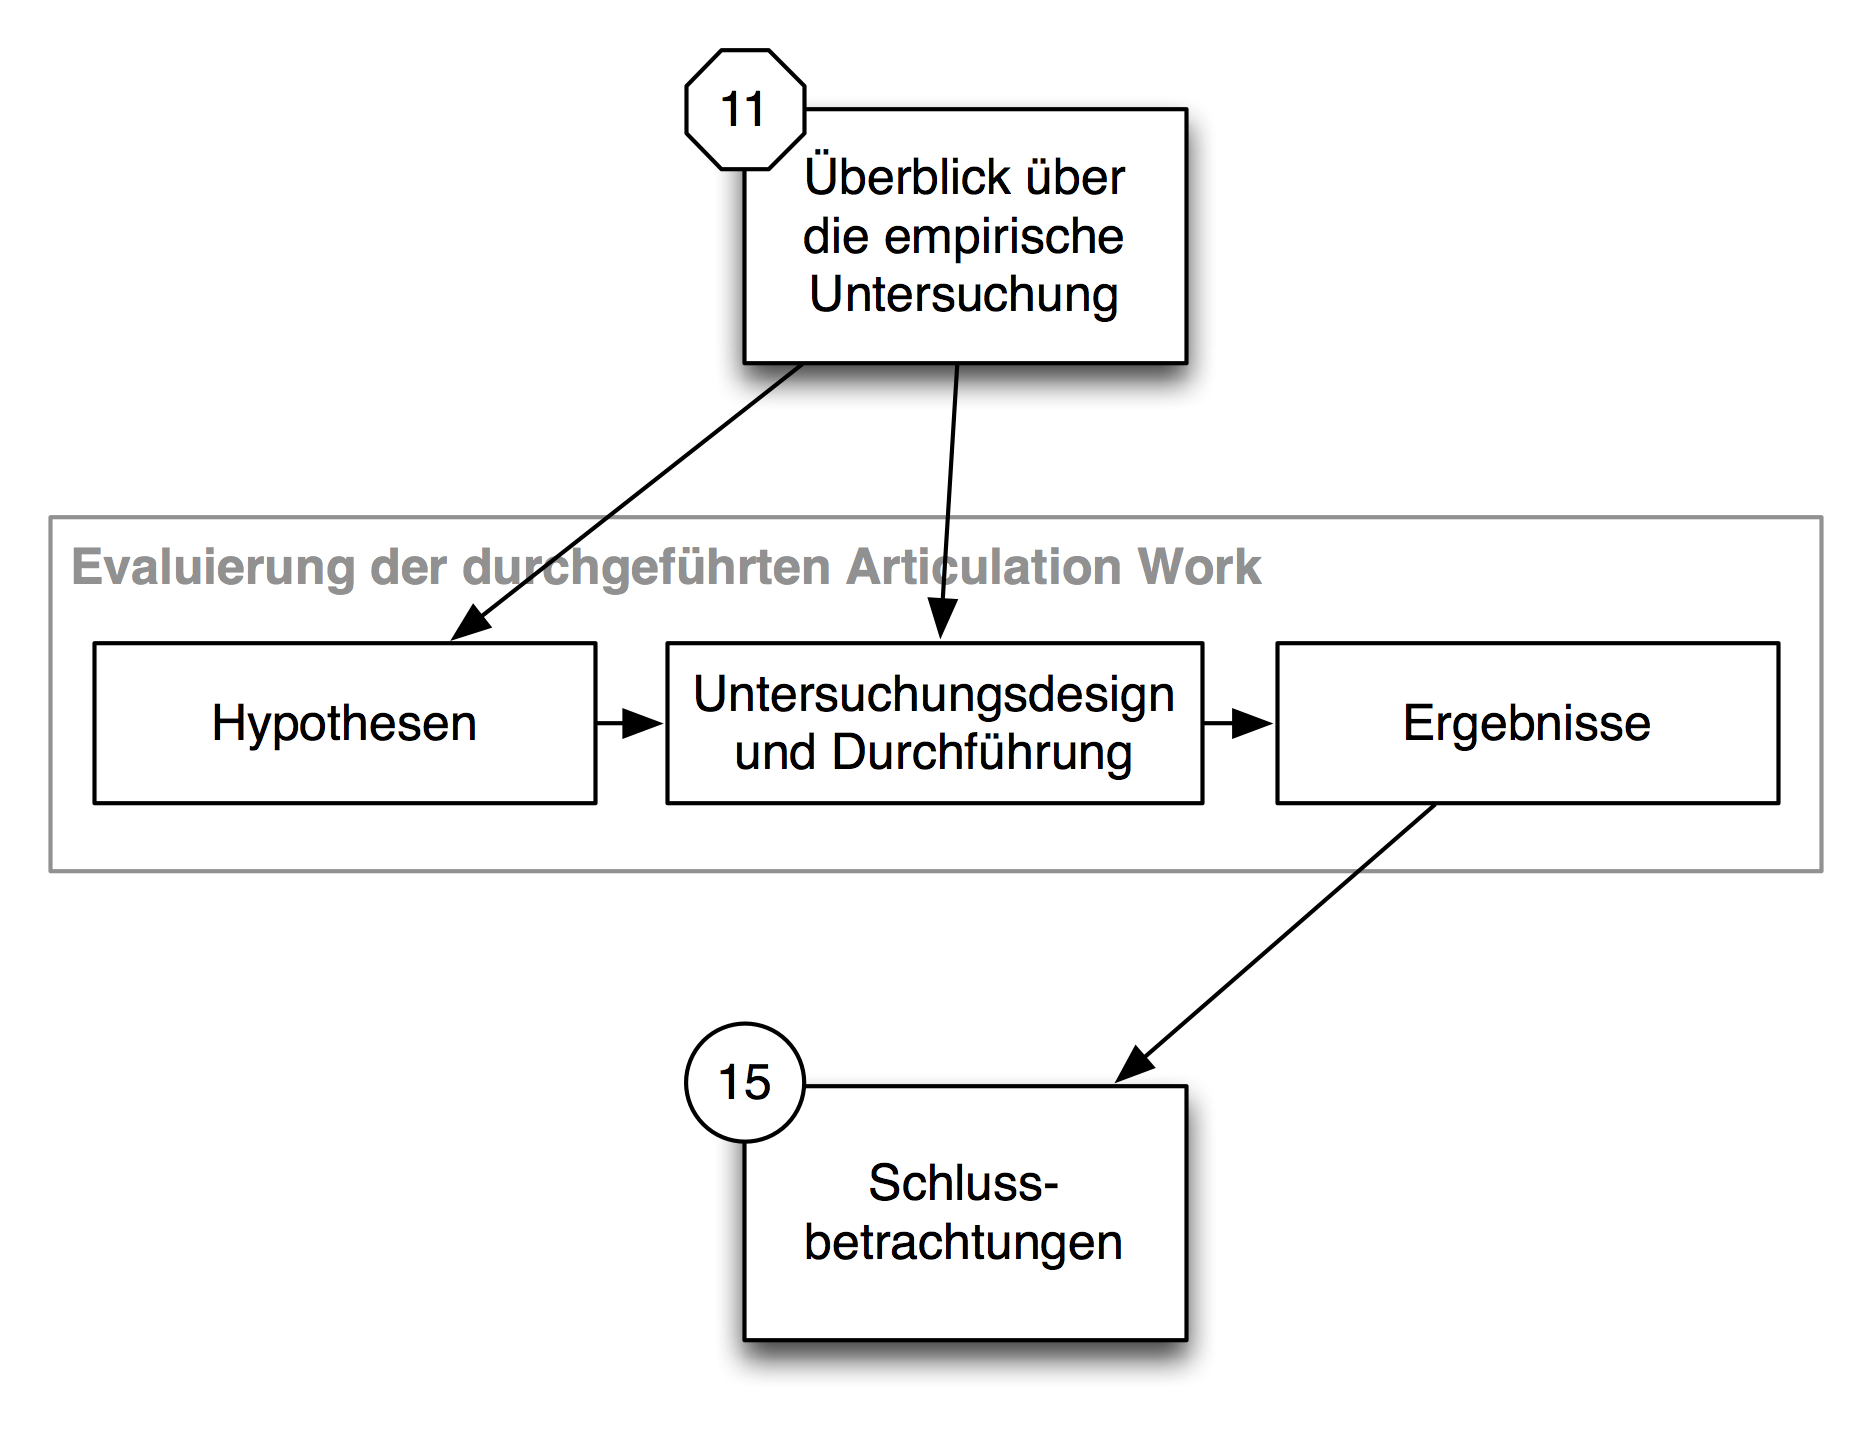
\includegraphics[scale=0.6]{img/Kontextgrafiken/k14.png}
	\caption{Kapitel „Evaluierung der durchgeführten Articulation Work“ im Gesamtzusammenhang}
	\label{fig:img_Kontextgrafiken_k14}
\end{figure}


Die in diesem Kapitel formulierten Hypothese basieren unmittelbar auf der Zielsetzung dieser Arbeit und den in Kapitel \ref{cha:articulation_work} identifizierten Merkmalen erfolgreich durchgeführter „Articulation Work“. Es wird nicht mehr auf die Verwendung der Werkzeugs selbst (siehe Kapitel \ref{cha:eval_werkzeug}) und nicht mehr auf die Rolle von externalisierten Modellen im Kontext dieser Arbeit (siehe Kapitel \ref{cha:eval_modell}) eingegangen.

\section{Hypothesen} % (fold)
\label{sec:a_hypothesen}

In diesem Abschnitt werden die Hypothesen angeführt und begründet, die in diesem Teil der empirischen Untersuchung geprüft werden. Die im Folgenden beschriebenen Hypothesen gehen aber auf die Wirkung von „Articulation Work“ auf die reale Welt ein. Nicht Gegenstand der Untersuchung ist die Verwendung diagrammatischer Modelle zum Zwecke der Durchführung von „Articulation Work“ (siehe \ref{cha:eval_modell}) und die Wirkung des Werkzeugs bei der Durchführung (siehe \ref{cha:eval_werkzeug}).

\subsection{Konzeptuell begründete Hypothesen} % (fold)
\label{sub:a_konzeptionell_begründete_hypothesen}

Die folgenden Hypothesen sind unmittelbar aus der globalen Zielsetzung dieser Arbeit abgeleitet. Die Wirkung von „Articulation Work“ zeigt sich in der organisationalen Realität an der Durchführung der „Production Work“ \citet{Fujimura87}. Um die Wirkung der mit dem Werkzeug durchgeführten „Articulation Work“ zeigen zu können, muss deshalb neben dieser auch die „Production Work“ betrachtet werden. Die Überprüfung erfolgt dabei in zwei Schritten. 

Im ersten Schritt wird die Durchführung der „Articulation Work“ selbst betrachtet. Im Rahmen der Verwendung der Externalisierung von mentalen Modellen zum Zwecke der Durchführung von „Articulation Work“ ist es -- wie in Kapitel \ref{cha:methodik} ausgeführt und in Anforderung \ref{anf:kollaborative_und_unmittelbare_manipulierbarkeit_des_modells} abgebildet -- notwendig, eine kooperative Nutzung des unterstützenden Werkzeugs zu ermöglichen. Ein wesentlicher Schritt zur erfolgreichen Durchführung von „Articulation Work“ ist neben der eigentlichen Externalisierung (die in den ersten beiden Hypothesen des vorhergehenden Kapitels \ref{cha:eval_modell} abgebildet wurde) die Abstimmung der indviduellen mentalen Modelle der Beteiligten. „Abstimmung“ bedeutet hier einen Abgleich der indviduellen Verständnisse jener Arbeitsaspekte, die im Sinne von Kapitel \ref{cha:articulation_work} „problematisch“ sind bzw. enge Kooperation der Beteiligten in der „Production Work“ bedingen. Die Prüfung dieser Hypothese ermöglicht die Beurteilung der Erfüllung der Anforderung \ref{anf:unterstützung_der_iterativen_aushandlung_des_modells} (siehe Seite \pageref{anf:unterstützung_der_iterativen_aushandlung_des_modells}).

\begin{hyp}
	\label{hyp:abstimmung}
	Das Werkzeug unterstützt den Prozess der Abstimmung der individuellen Modelle zwischen Personen.
\end{hyp}

Der zweite Schritt der Untersuchung in diesem Teil der Evaluierung betrachtet letztendlich die durchgeführte Arbeit selbst. Das globale Ziel des hier vorgestellten Ansatzes ist die Unterstützung von Articulation Work. Ob diese tatsächlich erfolgreich durchgeführt wurde, zeigt sich an der Wirkung auf die zugehörige kooperativer Arbeit (die „Production Work“). Es ist also zu beurteilen, ob die Anwendung des Werkzeuges tatsächlich auf die jeweils betrachteten Arbeitsabläufe wirkt und welcher Natur diese Auswirkungen sind. Die Prüfung dieser Hypothese ermöglicht die Beurteilung der Erfüllung der globalen Zielsetzung (siehe Seite \ref{zielsetzung}).

\begin{hyp}
	\label{hyp:wirkung}
	Die Anwendung des Werkzeugs hat Auswirkungen auf die Ergebnisse kooperativer Arbeit.
\end{hyp}

Hinsichtlich der in Kapitel \ref{cha:anforderungen} formulierten Anforderungen können die hier formulierten Hypothesen zusammenfassend wie in Tabelle \ref{tab:hyp_aw} dargestellt eingeordnet werden.

\begin{table}[htbp]
	\centering
	\caption{Hypothesen zu Articulation Work und deren Bezug zu den Anforderungen an das Werkzeug}
\begin{tabular}{|c|c|}
  \hline
   Hypothese & Anforderung \\ \hline
   \ref{hyp:abstimmung} & \ref{anf:unterstützung_der_iterativen_aushandlung_des_modells} \\
   \ref{hyp:wirkung} & globale Zielsetzung \\ \hline
\end{tabular} 
	\label{tab:hyp_aw}
\end{table}

% subsection konzeptionell_begründete_hypothesen (end)

% section hypothesen (end)

\section{Untersuchungsdesign und Durchführung} % (fold)
\label{sec:a_untersuchungsdesign}

In diesem Abschnitt wird auf Basis der oben formulierten Hypothesen das Untersuchungsdesign abgeleitet und die Durchführung der Untersuchung beschrieben. Der erste Teil des Abschnitts beschreibt die Operationalisierung der Hypothesen und damit die Festlegung wie diese konkret geprüft werden können. Im zweiten Teil des Abschnitts wird die Durchführung der Prüfung beschrieben. Hier erfolgt neben der Zuordnung der einzelnen Evaluierungsblöcke (siehe Abschnitt \ref{sec:globales_untersuchungsdesign}) auch die Darstellung rein beschreibender Modell-Parameter, die nicht unmittelbar in die Prüfung der Hypothesen eingehen. 

\subsection{Operationalisierung} % (fold)
\label{sub:a_operationalisierung}

In diesem Abschnitt wird für jede Hypothese identifiziert, in welcher Form sie geprüft werden kann. Dies umfasst die Festlegung der Messpunkte sowie der jeweiligen Mess- und Auswertungsmethode (letztere bezugnehmend auf den in Abschnitt \ref{sec:eingesetzte_werkzeuge_und_verfahren} beschriebenen Verfahren). Zudem werden jene Evaluierungsblöcke festgelegt, die für die jeweilige Untersuchung herangezogen wurden.

Für jede Hypothese wird also spezifiziert, anhand welcher Aspekte diese geprüft werden kann (= abhängige Variablen). Zudem wird festgelegt welche Ausgangssituation bei der Anwendung gewählt werden muss, um die Prüfung durchführen zu können (= unabhängige Variable) und welche Faktoren die Beurteilung ggf. ungewollt beeinflussen können (= Störvariablen).

\subsubsection{Abstimmung individueller Modelle} % (fold)
\label{ssub:abstimmung_individueller_modelle}

Gegenstand dieses Abschnitts ist die Prüfung der Hypothese \ref{hyp:abstimmung}. Diese bezieht sich auf die geforderte Eigenschaft des Werkzeugs, den Prozess der Abstimmung der individuellen Modelle zwischen den beteiligten Personen zu unterstützen.

Voraussetzung zur Prüfung dieser Hypothese ist, dass die Aufgabenstellung einem der beiden kooperativen Anwendungsszenarien zuzuordnen ist (siehe Abschnitt \ref{sub:abstimmung_individueller_mentaler_modelle} bzw. \ref{sub:aushandlung_individueller_mentaler_modelle}), in denen alle Teilnehmenden ihrer individuellen mentalen Modelle einbringen. Die Zielsetzung muss so formuliert sein, dass eine gemeinsame Sicht auf den behandelten Sachverhalt angestrebt wird. Weitere Voraussetzungen etwa hinsichtlich der Auswahl der beteiligten Individuen bestehen nicht.

Zur Prüfung, ob eine Abstimmung der individuellen Modelle der beteiligten Personen erreicht wurde, kann auf qualitative Beurteilung durch die Teilnehmenden zurückgegriffen werden. Zur Beurteilung bieten sich hier neben der direkten Frage nach der subjektiv wahrgenommene Abstimmung des Verständnisses auch Teilaspekte des \gls{PMS}-Framework \citep{Sedera02} an, das unter anderem die Wirkung der Modellbildung auf die beteiligten Personen und die Arbeitsrealität abbildet (zur Eignung des \gls{PMS}-Frameworks im Kontext dieser Arbeit siehe \citep{Wahlmuller10}).

Zusätzlich könnte zur Prüfung der Hypothese eine Diagnose der mentalen Modelle der Beteiligten etwa im Sinne von \citep{Ifenthaler06} durchgeführt werden. Hier müssten dann jeweils die externalisierten mentalen Modelle aller Beteiligten jeweils vor und nach dem Abstimmungsprozess gegenübergestellt werden. Die Anwendung dieses Vorgehens übersteigt jedoch den methodischen Fokus dieser Arbeit und wurde in der vorliegenden Untersuchung aus Ressourcengründen nicht durchgeführt.

% subsubsection abstimmung_individueller_modelle (end)

\subsubsection{Auswirkungen auf die Ergebnisse kooperativer Arbeit} % (fold)
\label{ssub:auswirkungen_auf_die_ergebnisse_kooperativer_arbeit}

Gegenstand dieses Abschnitts ist die Prüfung der Hypothese \ref{hyp:wirkung}. Diese bezieht sich letztendlich auf die Rückwirkung der mit Hilfe des Werkzeugs durchgeführten Aktivitäten auf die Realität.

Voraussetzung zur Prüfung dieser Hypothese ist, dass die Aufgabenstellung einen Sachverhalt zum Gegenstand hat, der eine unmittelbare Entsprechung in der realen (Arbeits-)Welt der Teilnehmenden hat. Weitere Voraussetzungen etwa hinsichtlich der Auswahl der beteiligten Individuen bestehen nicht.

Zur Prüfung dieser Hypothese kann wiederum auf eine qualitative Beurteilung der eingetretenen Veränderungen durch die beteiligten Personen zurückgegriffen werden. Auch hier liefert das \gls{PMS}-Framework \citep{Sedera02} wieder Ansatzpunkte zur Erhebung. Wichtig ist in diesem Zusammenhang die Einhaltung eines angemessenen zeitlichen Abstandes zwischen Modellbildung und Befragung, so dass etwaige Veränderungen in Kraft gesetzt bzw. beobachtete werden können.

Neben der Befragung der teilnehmenden Individuen können auch die Arbeitsabläufe, die Gegenstand der „Articulation Work“ waren, selbst beobachtet werden. Bei bereits etablierten Arbeitsabläufen bietet sich eine Gegenüberstellung der Durchführung der Arbeit vor und nach der Modellbildung an. Bei neu einzurichtenden Arbeitsabläufen steht die Möglichkeit der Gegenüberstellung nicht zur Verfügung. Dementsprechend kann lediglich beurteilt werden, ob die Aushandlung eines gemeinsamen Arbeitsablaufs möglich war. Vergleichend können im zweiten Fall dazu identische Arbeitsabläufe ohne dezidierten Abstimmungsschritt herangezogen werden, wobei als Maß für die Güte der Abstimmung die Anzahl der aufgetretenen Probleme in der Zusammenarbeit während der Durchführung der „Articulation Work“ herangezogen werden kann.

% subsubsection auswirkungen_auf_die_ergebnisse_kooperativer_arbeit (end)
% subsection a_operationalisierung (end)

\subsection{Durchführung} % (fold)
\label{sub:a_durchführung}

Die Durchführung der Untersuchungen zur diesem Teil der Evaluierung wurde in den Evaluierungsblöcken 2 und 4 durchgeführt. In Block 2 waren die Teilnehmenden aufgefordert, ein gemeinsames Vorgehen zur Erstellung einer Seminararbeit auszuhandeln und in einem zweiten, späteren Schritt zu reflektieren und ggf. anzupassen. Diese Schritte waren in den Verlauf der Erstellung der Seminararbeit eingebettet, begleiteten also die „Production Work“, an der der Erfolg der „Articulation Work“ zu messen war. Zur Beurteilung des Erfolgs wurden die Teilnehmenden aufgefordert den Verlauf der Erstellung der Seminararbeit in einem Prozess-Tagebuch zu dokumentieren und dabei besonders auf die Zusammenarbeit mit dem jeweiligen Partner einzugehen. Die Ergebnisse flossen in die Prüfung der Hypothese \ref{hyp:wirkung} ein.

In Block 4 wurden die Teilnehmer unmittelbar nach der Modellbildung und in einem Abstand von 8 Wochen zu den erwarteten bzw. tatsächlich eingetretenen Änderungen der Arbeitspraxis befragt. Die Befragung wurde mittels einem auf Basis des \gls{PMS}-Framework erstellten Fragebogen (siehe Anhang \ref{cha:daten_der_empirischen_untersuchung}) durchgeführt. Die Ergebnisse flossen in die Prüfung der Hypothesen \ref{hyp:abstimmung} und \ref{hyp:wirkung} ein.

In diesem Teil der Evaluierung wurden keine deskriptiven Parameter erhoben, weshalb die in den Kapiteln \ref{cha:eval_werkzeug} und \ref{cha:eval_modell} an dieser Stelle vorgenommene Beschreibung derselben hier entfällt.

\subsubsection{Stichprobe} % (fold)

Für die Untersuchung der Hypothesen in diesem Kapitel wurden die Evaluierungsblöcke 2 und 4 herangezogen.  In diesen war die Aufgabenstellung im Gegensatz zu den übrigen Evaluierungsblöcken stärker auf eine unmittelbare Abbildung konkreten Abläufen in der „Production Work“ ausgerichtet, was eine Prüfung der Hypothesen erleichterte. Für die Prüfung der Hypothese \ref{hyp:abstimmung} wären grundsätzlich auch die Evaluierungsblöcke 3 und 5 geeignet gewesen, die entsprechenden Untersuchungen konnten jedoch aus Ressourcengründen nicht durchgeführt werden. Die Stichprobe setzt sich wie in Tabelle \ref{tab:stichprobe_aw} beschrieben zusammen.

\begin{table}[htbp]
	\centering
	\caption{Stichproben der Evaluierung zur Articulation Work}

		\begin{tabular}{| l || c | c |}
		\hline
			Evaluierungsblock & $n_{Anwendungen}$ & $n_{Teilnehmende}$ \\ \hline
			Aushandlung 1 (1. Durchgang)  &  9 & 19 \\
			Aushandlung 1 (2. Durchgang)  &  9 & 18 \\
			Aushandlung 2				  & 10 & 13 \\ \hline
			Gesamt						  & 28 & 50 \\ \hline
	\end{tabular}
	\label{tab:stichprobe_aw}
\end{table}
% subsubsection stichprobe (end)

% subsection a_durchführung (end)
% section untersuchungsdesign (end)

\section{Ergebnisse} % (fold)
\label{sec:a_ergebnisse}

In diesem Abschnitt werden die Ergebnisse der Untersuchung gegliedert nach den oben formulierten Hypothesen dargestellt. Zu jeder Hypothese wird die Auswertung der empirischen Daten dargestellt, die Bedeutung der empirischen Belege für die Prüfung der jeweiligen Hypothese diskutiert und letztendlich das Ergebnis zusammenfassend dargestellt.  

\subsection{Abstimmung individueller Modelle} % (fold)
\label{sub:abstimmung_individueller_modelle}

Gegenstand der hier beschriebenen Untersuchung ist Hypothese \ref{hyp:abstimmung} („Das Werkzeug unterstützt den Prozess der Abstimmung der individuellen Modelle zwischen Personen.“). Als Grundlage dieser Untersuchung dienen die Ergebnisse der Evaluierungsblöcke 2 und 4.

\subsubsection{Auswertung} 

In Evaluierungsblock 4 wurden die Teilnehmer hinsichtlich der eigenen Einschätzung eines individuellen Erkenntnisgewinns bzw. der Entwicklung eines gemeinsamen Verständnisses befragt (Abschnitt „Auswirkungen der Modellierung“ im ersten und zweiten Fragebogen von Block 4  -- siehe Anhang \ref{sub:fb_eval4}). Die für die Prüfung der hier betrachteten Hypothese sind folgende geschlossene Items relevant:

\begin{enumerate}
	\item Die Modellierungstätigkeit hat mein Verständnis des Modellierungsinhalts erhöht.
	\item Die Modellierung hat Verbesserungen für bisherige Tätigkeiten aufgezeigt.
	\item Die Modellierung hat einen Beitrag zur Zielerreichung geleistet.
\end{enumerate}

Alle Fragen wurden sowohl in der unmittelbar nach der Modellbildung durchgeführten Befragung als auch in der in einem Abstand von 3 Monaten durchgeführten Befragung gestellt.

Insgesamt wurden in der unmittelbar nach der Modellbildung durchgeführten Befragung $n=14$ Teilnehmer befragt (1 Teilnehmer beantwortete die Fragestellungen nicht). Die Ergebnisse sind in Tabelle \ref{tab:verständnis} und Abbildung \ref{fig:img_Evaluierung_verständnis} zusammengefasst dargestellt. Neben dem Mittelwert und der Standardabweichung wurde für jedes Item auch geprüft, ob die Einschätzung als signifikant positiv zu bezeichnen ist. Dazu wurde ein einseitiger Signifikanz-Test für die Stichprobe gegenüber dem Skalenmittelwert 4 durchgeführt. Für die Items 1 und 2 konnte der t-Test angewandt werden, da die Stichprobe nicht signifikant von einer Normalverteilung abweicht (Shapiro-Wilk-Test: $W_{1}=0.894, p{1}=0.1103$, $W_{2}=0.8884, p{2}=0.0927$). Für Item 3 muss der Wilcoxon-Test angewandt werden, da die Stichprobe hier nicht normalverteilt ist (Shapiro-Wilk-Test: $W_{3}=0.6743, p{3}<0.005$).

\begin{table}[htbp]
	\centering
	\caption{Befragung über die Verständnisbildung bei der Modellierung -- Itemauswertung Teil 1}

\begin{tabular}{| c || c | c || c | c | c |}
  \hline
   Item & M & SD & $t_{M<4}$ & $V_{M<4}$ & $p_{M<4}$ \\ \hline
   1  & $2.615$ & $1.446$ & $-3.45$ & -- & $<0.005$ \\ 
   2  & $2.308$ & $1.032$ & $-5.92$ & -- & $<0.005$ \\ 
   3  & $2.417$ & $0.669$ & -- & $0$ & $<0.005$ \\ \hline
\end{tabular} \\ 
	\label{tab:verständnis}
\end{table}

\begin{figure}[htbp]
	\centering
		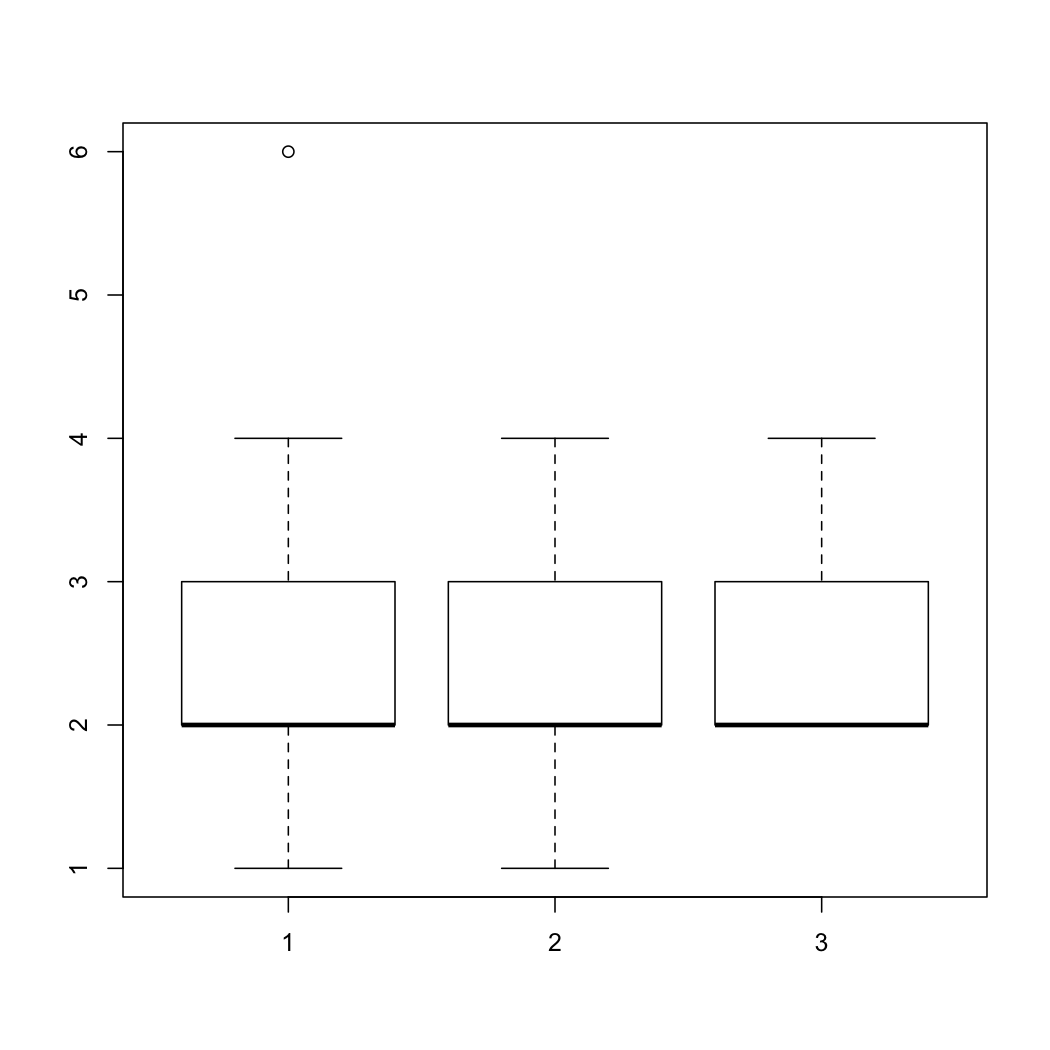
\includegraphics[height=2.5in]{img/Evaluierung/verstaendnis.png}
	\caption{Verteilung der Benutzereinschätzungen zur Verständnisbildung durch das Werkzeug -- Teil 1}
	\label{fig:img_Evaluierung_verständnis}
\end{figure}

Bei der drei Monate nach der Modellbildung durchgeführten Befragung beantworteten $n=11$ Teilnehmer die Fragestellungen. Die Ergebnisse sind in Tabelle \ref{tab:verständnis2} und Abbildung \ref{fig:img_Evaluierung_verständnis2} zusammengefasst dargestellt. Für die Signifikanzprüfung der Items konnte der t-Test angewandt werden, da die Stichprobe in allen drei Fällen nicht signifikant von einer Normalverteilung abweicht (Shapiro-Wilk-Test: $W_{1}=0.854, p{1}=0.0486$, $W_{2}=0.924, p{2}=0.353$, $W_{3}=0.893, p{3}=0.150$).

\begin{table}[htbp]
	\centering
	\caption{Befragung über die Verständnisbildung bei der Modellierung -- Itemauswertung Teil 2}

\begin{tabular}{| c || c | c || c | c |}
  \hline
   Item & M & SD & $t_{M<4}$ & $p_{M<4}$ \\ \hline
   1  & $2.818$ & $1.168$ & $-3.36$ & $<0.005$ \\ 
   2  & $2.909$ & $1.221$ & $-2.96$ & $<0.005$ \\ 
   3  & $2.455$ & $0.820$ & $-6.25$ & $<0.005$ \\ \hline
\end{tabular} \\ 
	\label{tab:verständnis2}
\end{table}

\begin{figure}[htbp]
	\centering
		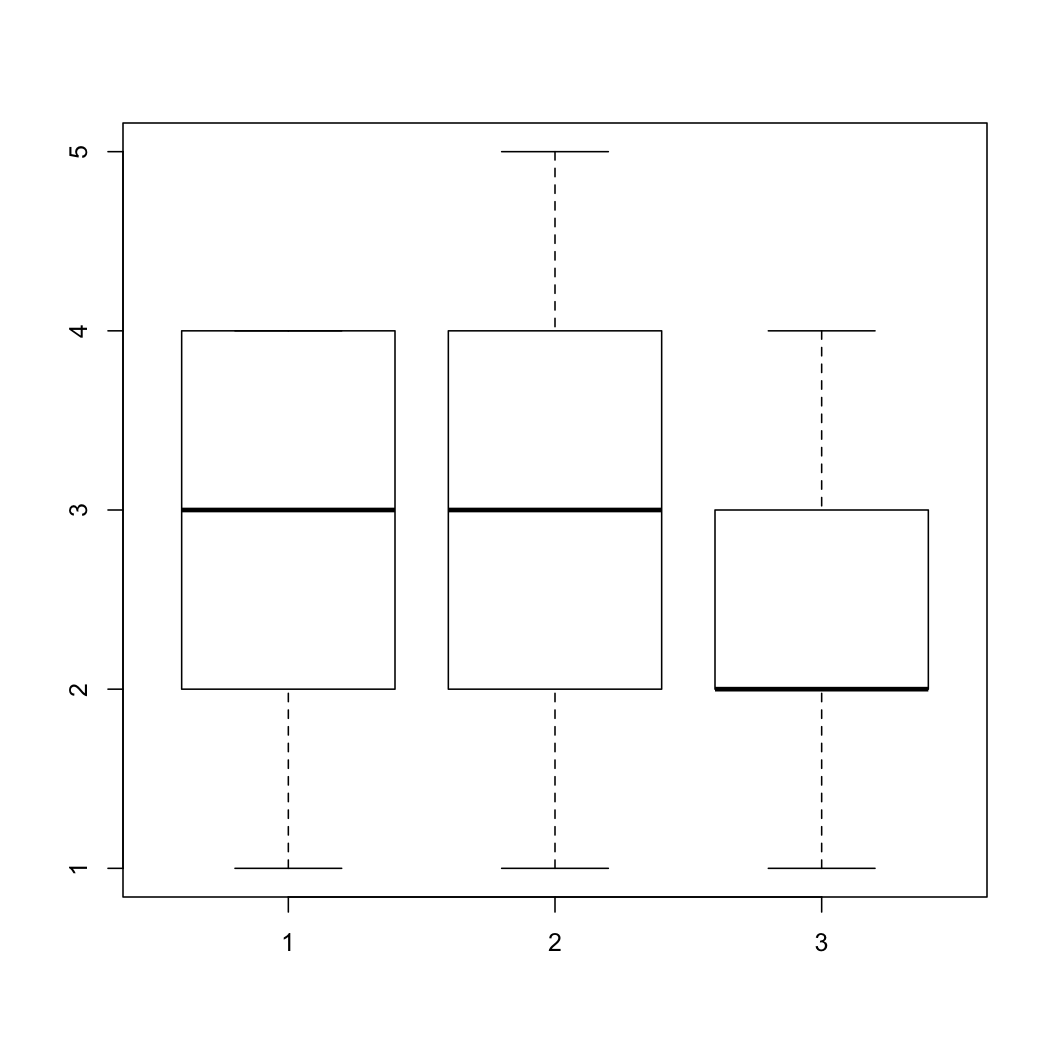
\includegraphics[height=2.5in]{img/Evaluierung/verstaendnis2.png}
	\caption{Verteilung der Benutzereinschätzungen zur Verständnisbildung durch das Werkzeug -- Teil 2}
	\label{fig:img_Evaluierung_verständnis2}
\end{figure}

Vergleicht man die Antworten in den beiden Fragebögen, so ergibt sich für keines der Items ein signifikanter Unterschied in der Bewertung (zweiseitiger Signifikanztest für ungepaarte Stichproben: $t_{1}=-0.380, p_{1}=0.708$, $t_{2}=-1.29, p_{2}=0.212$, $W_{3}=62.5, p_{3}=0.836$\footnote{Bei Item 3 musste aufgrund der Nicht-Normalverteilung der Stichprobe aus dem ersten Fragebogen der Wilcoxon-Test angewandt werden, für die anderen beiden Items konnte ein t-Test durchgeführt werden}).

In den Evaluierungsblöcken 4 und 5 wurden die Teilnehmer ($n=37$) außerdem in offenen Fragen nach der Zusammenarbeit im Team befragt (Fragestellung: „Wie würden Sie Ihre Beziehung im Team beschreiben?“ sowie „Sind Sie zufrieden mit ihrem Beitrag zum Modellierungsprozess? Geben Sie bitte auch eine kurze Begründung an!“) -- siehe dazu auch die Auswertungen in Abschnitt \ref{sub:wirkung_auf_die_kooperation_bei_der_modellerstellung}). Während diese nicht unmittelbar auf die hier betrachtete Hypothese eingehen, gaben doch 12 Teilnehmer explizit an, dass ein Konsens über die abzubildenden Inhalte gefunden werden konnte. 7 dieser 12 Teilnehmer führten außerdem an, dass während der Modellierung Meinungsverschiedenheiten geherrscht hätten, die aufgelöst werden konnten.

In der Auswertung der Videoaufnahmen der Evaluierungsblöcke 2 bis 5 (in denen kooperative Modellbildungen durchgeführt wurden, $n=69$) waren insgesamt 53 Situationen zu identifizieren, in denen die Teilnehmer bei der Abbildung eines Sachverhaltes offensichtlich unterschiedlicher Meinung waren. Vier unterschiedliche Reaktionen waren als Konsequenz zu beobachten:
\begin{enumerate}
	\item Eine unterschiedliche Meinung wurde übergangen, lediglich die andere Meinung fand sich im Modell wieder. (10x)
	\item Die unterschiedlichen Meinungen wurden nicht explizit aufgelöst, fanden sich jedoch beide im Modell wieder. (5x)
	\item Der Sachverhalt, in dem unterschiedliche Meinungen herrschten, wurde im Modell nicht abgebildet. (17x)
	\item Die Teilnehmer fanden zu einer gemeinsamen Sichtweise und bildeten diese im Modell ab. (21x)
\end{enumerate}
  
\subsubsection{Diskussion} 

In den dezidierten Fragestellungen etwaigen Auswirkungen der Werkzeugverwendung auf das Verständnis der Teilnehmer in Evaluierungsblock 4 zeigte sich durchgängig eine signifikant positive Einschätzung der Veränderungen. Die Frage nach der „Erhöhung des indiviuduellen Verständnisses des modellierten Sachverhalts“ ist dabei bei der Beurteilung der hier betrachteten Hypothese als am relevantesten einzuschätzen. Auch das „Aufzeigen von Verbesserungspotential in der Modellierung“ impliziert die Zusammenführung der individuell wahrgenommenen Aspekte des modellierten Sachverhalts, eine positive Einschätzung dieser Fragestellung stützt also ebenfalls die Hypothese. Auch die Frage, ob die Modellbildung einen „Beitrag zur Zielerreichung“ geleistet hätte, ist unter der Annahme relevant, das die Zielsetzung (wie in Block 4 gegeben) explizit die Forderung nach dem Sichtbarmachen der eignen Sichtweise sowie der Entwicklung einer gemeinsamen Sichtweise enthielt. In der mittelfristigen Betrachtung drei Monate nach deer Modellbildung zeigt sich keine signifikante Änderung der Einschätzung und bleibt für alle drei Fragen signifikant positiv. Die Ergebnisse der betrachteten geschlossenen Fragen stützen also die oben formulierte Hypothese.

In den relevanten offenen Fragen wurde von den Teilnehmern der Evaluierungsblöcke 4 und 5 in etwa einem Drittel der Antworten auf die Konsensbildung als einen wichtigen Aspekt der Werkzeugverwendung verwiesen. Dies erscheint insofern als relevant für die Unterstützung der hier formulierten Hypothese, da die Fragen vollständig offen formuliert waren und keine andere Wirkung des Werkzeugs in diesem Ausmaß erwähnt wurde. Einschränkend ist zu bemerken, dass bei den Werkzeuganwendungen durchgängig nicht hoch kontroversielle Themen behandelt wurden. Etwa ein Fünftel aller Teilnehmer (bzw. die Hälfte der Teilnehmer, die konsensbildende Wirkung genannt hatten) führte an, dass Meinungsverschiedenheiten in unterschiedlichem Ausmaß bestanden hätten, die ausgeräumt werden konnten. Im Falle der Modellbildung mit dem Werkzeug CMapTools in Evaluierungsblock 5 wurde bei insgesamt 24 befragten Teilnehmern hingegen zweimal explizit angeführt, dass ein Teilnehmer inhaltlich dominiert hätte und der andere sich nicht einbringen konnte (siehe Abschnitt \ref{sub:wirkung_auf_die_kooperation_bei_der_modellerstellung}), dessen Sichtweise also auch nicht in eine gemeinsame Sichtweise hätte einfließen können.

In den Auswertungen der Videoaufnahmen konnten ebenfalls Situationen identifiziert werden, in denen offenbar Meinungsverschiedenheiten in unterschiedlichem Ausmaß hinsichtlich der Abbildung herrschten. In etwa 40\% der identifizierten Fälle fanden die Teilnehmer zu einer gemeinsamen Sichtweise, die im Modell abgebildet wurde (Fall 4). In etwa einem Drittel der Fälle wurde die Meinungsverschiedenheit ignoriert und im Modell nicht abgebildet (Fall 3). In einem Fünftel der Fälle wurden konfliktionierende Sichtweisen übergangen und nur eine Variante fand ohne weitere Diskussion den Weg in das Modell (Fall 1). Ein weiteres Zehntel der Meinungsverschiedenheiten wurde ebenfalls nicht explizit angesprochen, die Sichtweisen wurden jedoch gleichberechtigt in das Modell aufgenommen (Fall 2). Fall 4 und Fall 2 stützen die Hypothese, während Fall 3 und Fall 1 eher für deren Ablehnung sprechen. Insgesamt zeigen also etwa 50\% der Fälle Ausprägungen, die die Hypothese unterstützen.   

Insgesamt überwiegen also jene Untersuchungsergebnisse, die die Annahme der Hypothese unterstützen. Sie kann also auf Basis der durchgeführten Untersuchung bestätigt werden, bedarf aber weiterführender Untersuchungen hinsichtlich des auffällig häufig auftretenden Benutzerverhaltens des Aussparens unterschiedlicher Sichtweisen in der Diskussion.

\subsubsection{Ergebnis} 

\textbf{Die Hypothese \ref{hyp:abstimmung} kann auf Basis der Untersuchung bestätigt werden.} Sowohl die quantitativen als auch die qualitativen Daten der Benutzerbefragung stützen die Hypothese und sprechen für deren Annahme. In der Auswertung der durchgeführten Modellbildungen zeigte sich keine signifikante Häufung von die Hypothese stützendem Umgang mit unterschiedlichen Sichtweisen. Auffällig häufig wurden die Aspekte, in denen unterschiedliche Sichtweisen herrschten, nicht weiter angesprochen und im Modell ausgespart. Dieses Verhalten bedarf weiterführenden Untersuchungen bzw. der Entwicklung von methodischen Ansätzen, die die Auflösung von derartigen Situationen erleichtern bzw. bestärken.

% subsection abstimmung_individueller_modelle (end)

\subsection{Auswirkungen auf die Ergebnisse kooperativer Arbeit} % (fold)
\label{sub:auswirkungen_auf_die_ergebnisse_kooperativer_arbeit}

Gegenstand der hier beschriebenen Untersuchung ist Hypothese \ref{hyp:wirkung} („Die Anwendung des Werkzeugs hat Auswirkungen auf die Ergebnisse kooperativer Arbeit.“). Als Grundlage dieser Untersuchung dienen die Ergebnisse der Evaluierungsblöcke 2 und 4.

\subsubsection{Auswertung} 

In Evaluierungsblock 4 wurden die Teilnehmer hinsichtlich der eigenen Einschätzung der Auswirkungen der Modellbildung auf die reale Arbeitswelt („Production Work“) drei Monate nach der Durchführung der Modellbildung befragt (Abschnitt „Auswirkungen auf die Prozesse“ im zweiten Fragebogen von Block 4 sowie Abschnitt  -- siehe Anhang \ref{sub:fb_eval4}). Die für die Prüfung der hier betrachteten Hypothese sind folgende geschlossene Items relevant:

\begin{enumerate}
	
	\item Umsetzung
		\begin{enumerate}
			\item Das Modellierungsergebnis oder Teile davon wurden bereits umgesetzt.
			\item Das Modellierungsergebnis oder Teile davon werden in Kürze umgesetzt.
			\item Es ist geplant die Modellierungsergebnisse oder Teile davon umzusetzen.
		\end{enumerate}
	\item Der Alltag hat sich im Umfeld des modellierten Themas geändert.
	\item Unmittelbar nach der Modellierung war klar, dass die Ergebnisse umgesetzt werden.
\end{enumerate}

Insgesamt wurden in der drei Monate nach der Modellbildung durchgeführten Befragung 11 Teilnehmer befragt (5 Teilnehmer beantworteten alle Fragestellungen nicht, 5 Teilnehmer beantworteten alle Fragestellungen, 1 Teilnehmer beantwortete nur die drei Items der Fragestellung 1). Die Ergebnisse sind in Tabelle \ref{tab:wirkung} und Abbildung \ref{fig:img_Evaluierung_wirkung} zusammengefasst dargestellt. Für die drei unter Punkte 1 gruppierten Items wird einerseits eine Einzelauswertung vorgenommen, andererseits werden diese Items so gruppiert, dass jeweils der geringste Wert (also die „beste“ Einschätzung) verwendet wird. So ist es möglich, ein Maß für die generelle Wahrnehmung der Umsetzung des Modellierungsergebnisses zu bestimmen.

Neben dem Mittelwert und der Standardabweichung wurde für jedes Item auch geprüft, ob die Einschätzung als signifikant unterschiedlich von Skalenmittelwert 4 zu bezeichnen ist. Dazu wurde ein zweiseitiger Signifikanz-Test für die Stichprobe gegenüber dem Skalenmittelwert 4 durchgeführt. Aufgrund der geringen Stichprobengröße wurde der Wilcoxon-Test zur Signifkanzprüfung verwendet.

\begin{table}[htbp]
	\centering
	\caption{Befragung über die Wirkung der Modellbildung auf die Arbeitsprozesse -- Itemauswertung}

\begin{tabular}{| c || c | c | c || c | c |}
  \hline
   Item & n & M & SD & $V_{M=4}$ & $p_{M=4}$ \\ \hline
   1a         & 6 & $3.83$ & $1.941$ & $2.5$ & $1$ \\ 
   1b         & 6 & $3.33$ & $2.066$ & $4.5$ & $0.496$ \\ 
   1c         & 6 & $3.50$ & $2.074$ & $3.5$ & $0.713$ \\ 
   $1_{ges}$  & 6 & $3.33$ & $2.066$ & $4.5$ & $0.496$ \\ 
   2          & 5 & $4.40$ & $1.673$ & $4$ & $0.773$ \\ 
   3          & 5 & $3.40$ & $0.548$ & $0$ & $0.149$ \\ \hline
\end{tabular} \\ 
	\label{tab:wirkung}
\end{table}

\begin{figure}[htbp]
	\centering
		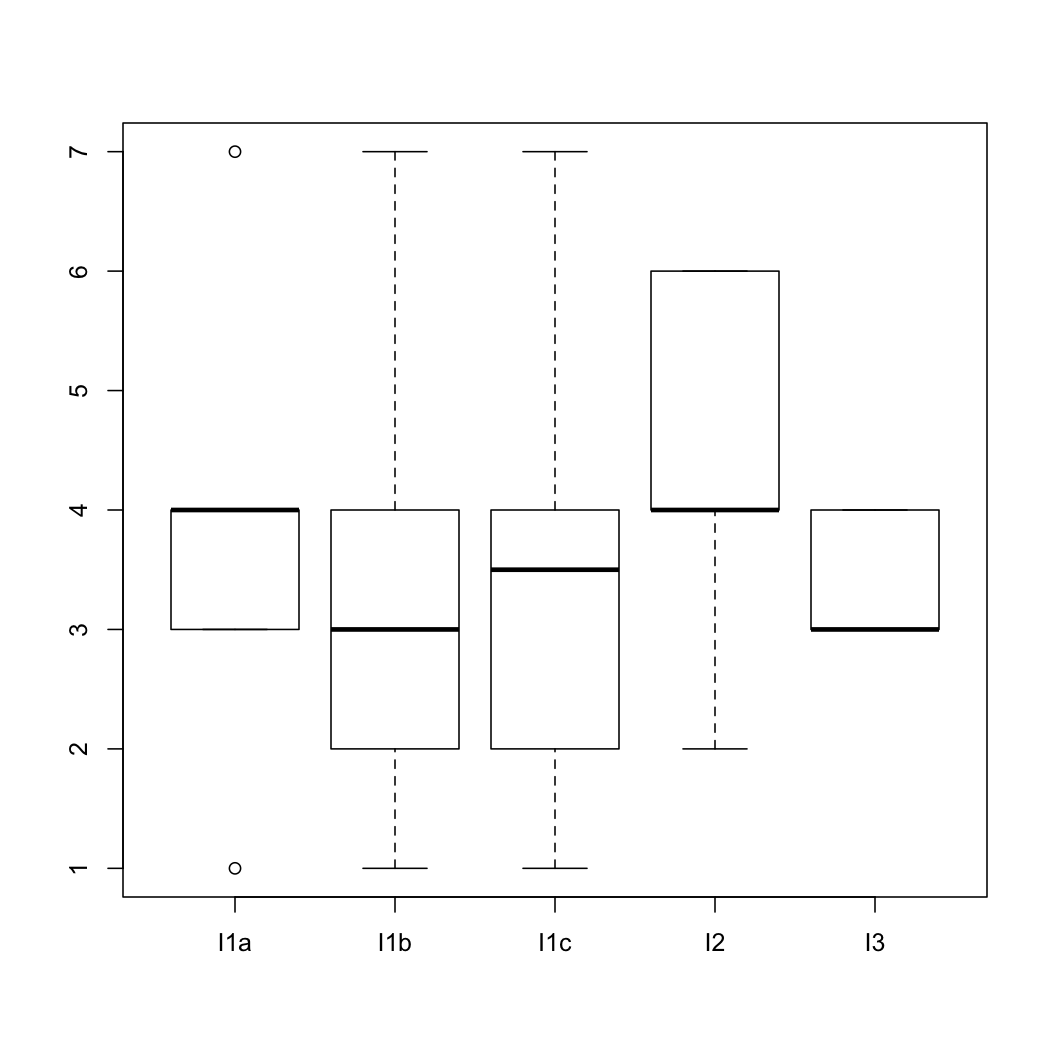
\includegraphics[height=2.5in]{img/Evaluierung/wirkung.png}
	\caption{Verteilung der Benutzereinschätzungen zur Wirkung der Modellbildung auf die Arbeitsprozesse}
	\label{fig:img_Evaluierung_wirkung}
\end{figure}

In keinem der Items konnte eine signifikante Abweichung vom Skalenmittelwert 4 gemessen werden, was einer neutralen Antwort entspricht (Skala: 1 \ldots „stimme zu“, 7 \ldots „stimme nicht zu“). 5 bzw. 6 Teilnehmer gaben explizit keine Antwort (Antwortmöglichkeit „keine Antwort“).

In den offenen Fragen des Fragebogenteils nutzten 4 Teilnehmer die Gelegenheit zu weiteren Kommentaren. Aufgrund des geringen Rücklaufs wird auf eine Codierung der Antworten verzichtet, es werden für jede offene Frage die Antworten im Volltext angeführt (in Klammern sind die Quellfragebögen der Antworten angeführt):

\begin{itemize}
	\item „Welche Ergebnisse hatte die Modellierung“ \\
		\begin{enumerate}
			\item Erarbeitung / Verbesserung von Prozessen \& Dokumentationen (FB2)
			\item klare Definition des systemischen Soll‐Zustandes (FB2)
			\item generell mehr Klarheit bei den Beteiligten zum Thema (FB2)
			\item Darstellung der kritischen Punkte im Prozess (FB4)
			\item wir kamen leider nicht so weit, ein Ergebnis festzuhalten bzw. ein Ziel zu formulieren (FB5)
			\item Erhöhtes Verständnis der hohen Komplexität des Systems. (FB11) 
		\end{enumerate}
	\item „Welche Auswirkungen konnten Sie persönlich feststellen?“ \\
		\begin{enumerate}
			\item Diskussion / Neue Wege (FB4)
			\item Es war nett, ein solches Tool kennen zu lernen, es hatte aber keine Auswirkungen für mich persönlich (FB5)
			\item Mehr Verständnis bei Umsetzungen, die Komplexität wurde durch das Tool transparenter (FB11) 
		\end{enumerate}
	\item „Welche Auswirkungen erwarten Sie“ \\
		\begin{enumerate}
			\item zu den bisherigen Umsetzungsmaßnahmen die weitere operative Umsetzung der gewonnenen Erkenntnisse (FB2)
			\item Verbesserung im Prozess: kürzere Wege, Nachvollziehbarkeit (FB4)
		\end{enumerate}
\end{itemize}

In Evaluierungsblock 2 wurde versucht, die Wirkung des Werkzeugs unmittelbar an der „Production Work“ zu messen. Dazu wurde zum Ersten der Ablauf der „Production Work“ von den Teilnehmern dokumentiert. Zum Zweiten wurden die Ergebnisse der „Production Work“, im Fall dieses Evaluierungsblocks also die erstellten Seminararbeiten ausgewertet. Dabei wurde neben der inhaltlichen Beurteilung vor allem auch auf die Konsistenz der erstellten Arbeit geachtet. Ist diese bei mehreren Autoren gegeben, so ist dies ein Indikator für die erfolgreiche Durchführung von „Articulation Work“. Die Arbeiten, die im Rahmen des Evaluierungsblocks 2 erstellt wurden, wurden zudem den Arbeiten eines Seminars gegenüber gestellt, in dem eine identische Aufgaben- und Themenstellung ohne Einsatz einer expliziten Unterstützung von „Articulation Work“ bearbeitet wurde.

Insgesamt wurden in Evaluierungsblock 10 Arbeiten erstellt, an denen 20 Teilnehmer beteiligt waren. In 8 Fällen arbeiteten jeweils 2 Teilnehmer zusammen, in je einem Fall arbeiteten 3 Personen bzw. 1 Person an der Arbeit.

Zur Auswertung der Ergebnisse der „Production Work“ wird einerseits die Gesamtbeurteilung der Arbeit auf einer Notenskala von 1 („sehr gut“) bis 5 („nicht genügend“) angegeben\footnote{In die Gesamtbeurteilung fließen die inhaltliche Qualität der Arbeit, deren Konsistenz („roter Faden“) sowie die Aufbereitung der Inhalte (inkl. Formulierungen und Korrektheit der Quellen-Referenzierung) ein}. Andererseits wird explizit eine Einschätzung der Qualität der Konsistenz ebenfalls auf einer Skala von 1 bis 5 angeführt. Beide Werte wurden durch den Lehrveranstaltungsleiter festgelegt, der gleichzeitig auch der Autor dieser Arbeit ist. In Tabelle \ref{tab:ergebnis} ist das Ergebnis der Beurteilung für die Durchführung in Evaluierungblock 2 (unter Einsatz des hier vorgestellten Werkzeugs) dargestellt. In Tabelle \ref{tab:ergebnis_ohne} ist das Ergebnis eines inhaltlich identischen Seminars dargestellt, in dem der Ablauf nur durch den fehlenden Einsatz des Werkzeugs von dem in der ersten Tabelle dargestellten Seminar abwich. 

\begin{table}[htbp]
	\centering
	\caption{Ergebnis der „Production Work“ in Evaluierungsblock 2}

\begin{tabular}{| c || c || c | c |}
  \hline
   Arbeit & Teilnehmer & $Note_{ges}$ & $Note_{Konsistenz}$ \\ \hline
   1         & 2 & 2 & 2 \\ 
   2         & 2 & 3 & 4 \\ 
   3         & 2 & 1 & 1 \\ 
   4         & 1 & 2 & 1 \\ 
   5         & 2 & 2 & 2 \\ 
   6         & 2 & 2 & 3 \\ 
   7         & 2 & 1 & 1 \\ 
   8         & 3 & 1 & 1 \\ 
   9         & 2 & 2 & 3 \\ 
   10        & 2 & 2 & 2 \\ \hline
\end{tabular} \\ 
	\label{tab:ergebnis}
\end{table}

\begin{table}[htbp]
	\centering
	\caption{Ergebnis der „Production Work“ ohne Unterstützung der „Articulation Work“}

\begin{tabular}{| c || c || c | c |}
  \hline
   Arbeit & Teilnehmer & $Note_{ges}$ & $Note_{Konsistenz}$ \\ \hline
   1         & 2 & 1 & 1 \\ 
   2         & 2 & 2 & 3 \\ 
   3         & 2 & 2 & 3 \\ 
   4         & 2 & 1 & 1 \\ 
   5         & 2 & 2 & 4 \\ 
   6         & 2 & 3 & 4 \\ 
   7         & 1 & 1 & 1 \\ 
   8         & 1 & 3 & 4 \\ 
   9         & 2 & 3 & 4 \\ 
   10        & 2 & 1 & 1 \\ \hline
\end{tabular} \\ 
	\label{tab:ergebnis_ohne}
\end{table}

Insgesamt konnte hinsichtlich der Konsistenz der Arbeiten bei der Durchführung des Seminars mit Unterstützung der durchgeführten „Articulation Work“ ($M=2.0, SD=1.05$) gegenüber jener ohne Unterstützung ($M=2.6, SD=1.43$) keine statistisch signifikante Verbesserung des Ergebnisses festgestellt werden (einseitiger Wilcoxon-Test für ungepaarte Stichproben: $W=38, p=0.181$\footnote{Der Wilcoxon-Test musste angewandt werden, da die Stichprobe der Durchführung ohne Werkzeugunterstützung nicht normalverteilt ist (Shaprio-Wilk-Test: $W=0.752, p<0.005$)}). Auch das Gesamtergebnis ist bei Unterstützung der „Articulation Work“ ($M=1.8, SD=0.63$) nicht signifikant besser (einseitiger Wilcoxon-Test für ungepaarte Stichproben: $W=47.5, p=0.435$) als jenes ohne Unterstützung ($M=1.9, SD=0.87$). In dem Seminar, das ohne Unterstützung des Werkzeugs durchführt wurde, zerbrach eine Gruppe aufgrund von unüberbrückbaren Meinungsverschiedenheiten. Dies war durchgängig auch in insgesamt 6 betrachteten in vorhergehenden Semestern und parallel durchgeführten Seminaren in jeweils 1 bis 2 von 10 bis 12 Gruppen der Fall. In dem mit Unterstützung des hier vorgestellten Werkzeugs durchgeführten Seminar wurde keine Gruppe aufgelöst, alle Gruppen bestanden trotz der zufälligen Zuteilung der Partner bis zum Ende des Seminars.

In der Dokumention der „Production Work“ durch die Teilnehmer des Evaluierungsblocks 2 wird untersucht, welche Vorgehensweise bei der Zusammenarbeit bei der Erstellung der Seminararbeit gewählt wurde. Diese wird den erstellten Modellen gegenübergestellt. Dabei wird untersucht ob die tatsächliche Vorgehensweise dem bei der Durchführung der „Articulation Work“ vereinbarten Prozedere entspricht. Zusätzlich werden etwaige Anmerkungen hinsichlich problematischer Kooperation und Referenzen auf die Auswirkungen der „Articulation Work“ angeführt.

\paragraph{Arbeit 1} % (fold)
\label{par:arbeit_1}

Die Teilnehmer teilten die inhaltliche Arbeit unter sich auf und arbeiten die einzelnen Blöcke eigenständig aus. Die einzelnen Teile wurden zu zwei Zeitpunkten (nach der Literaturrechereche und nach der Erstellung d er Draft Version) gemeinsam konsolidiert. An die Draft-Version schloss sich eine kooperative Bearbeitung des Gesamtdokuments an, in der die Gesamtdurchgängigkeit der Arbeit sichergestellt wurde. Dieses Vorgehen stimmt mit dem in der Modellbildung vereinbarten Vorgehen überein. Hinsichtlich der Durchführung wurden keine Probleme oder Auffälligkeiten angeführt. Resümierend merken beide Teilnehmer an, dass der Großteil der inhaltlichen Arbeit individuell erfolgte und die Druchgängigkeit der Inhalte darunter litt.

% paragraph arbeit_1 (end)

\paragraph{Arbeit 2} % (fold)
\label{par:arbeit_2}

Die Teilnehmer treffen in der Dokumentation keine explizite Aussage zur Arbeitsteilung, scheinen aber das Thema inhaltlich aufgeteilt und jeweils separat bearbeitet zu haben. Aus den erstellen Modellen wäre grundsätzlich ein Vorgehen zu erkennen, dass individuelle Teilarbeiten mit regelmäßigen Abgleichsaktivitäten spezifiziert. Dieses scheint jedoch nicht umgesetzt worden zu sein. Ein Teilnehmer beschreibt Uneinigkeiten in der Ablaufplanung, die noch aufgelöst werden müssten. Der andere Teilnehmer führt retrospektiv an, dass die Arbeit von zu hoher Arbeitslast in anderen Fächern des Studiums negativ beeinflusst gewesen wäre.  

% paragraph arbeit_2 (end)

\paragraph{Arbeit 3} % (fold)
\label{par:arbeit_3}

Die Teilnehmer dokumentieren ein ab dem Beginn des Schreibprozessen ein eher separiertes Vorgehen bei der Erstellung der Seminararbeit. Die Literaturrecherche wurde inhaltlich noch nicht abgrenzt, wurde aber von beiden Teilnehmern individuell durchgeführt. In der Modellierung wurde die Aushandlung eines konkreten Vorgehens ausgespart, vielmehr berichtete ein Teilnehmer über das Vorgehen bei einem ähnlichen Seminar im Vorjahr. Dieses Modell schien jedoch bei der konkreten Durchführung nicht mehr berücksichtigt zu werden. Bei der Erstellung scheint ein Teilnehmer die Führung in der Zusammenstellung der einzelnen Teile übernommen zu haben. Dieser Teilnehmer dokumentiert auch eine positive Wahrnehmung der Zusammenarbeit, während der andere Teilnehmer von Kommunikationsproblemen und ungerechtfertigt erscheinenden Kürzungen seiner Beiträge in der Gesamtarbeit berichtet. 
% paragraph arbeit_3 (end)

\paragraph{Arbeit 4} % (fold)
\label{par:arbeit_4}

Diese Arbeit wurde individuell von nur einem Teilnehmer erstellt. In der Dokumentation nimmt der Ersteller keinen Bezug auf das erstellte Modell, das Vorgehen scheint jedoch kohärent mit dem bei der Modellerstellung geplanten Vorgehen zu sein.
% paragraph arbeit_4 (end)

\paragraph{Arbeit 5} % (fold)
\label{par:arbeit_5}

Die Teilnehmer kennen einander von früheren Projekten und haben bereits zusammengearbeitet. Die Kooperation wird als problemlos bezeichnet, den inhaltlich aufgeteilten eigenständigen Arbeitsphasen folgen regelmäßig gemeinsame Konsolidierungsschritte, die Teilnehmer halten sich gegenseitig über den aktuellen Stand der Arbeit am Laufenden. Die dokumentierte Zusammenarbeit lässt auf eine stärkere Interaktion als ursprünglich in der Modellierung geplant schließen.

% paragraph arbeit_5 (end)

\paragraph{Arbeit 6} % (fold)
\label{par:arbeit_6}

Die Teilnehmer teilten die Arbeit inhaltlich in zwei Teile und bearbeiteten diese individuell. Die Integration wurde zweimal durchgeführt (Draft Version, Finale Version), dies wurde jeweils abwechselnd von einem der Teilnehmer durchgeführt. Vor der Abgabe wurde eine gemeinsame Konsolidierung mit web-basierten Werkzeugen synchron durchgeführt. Das erstellte Modell zeigt keinen Ablaufplan, sondern gibt die inhaltliche Aufteilung der Arbeit wieder. Diese entspricht der in der Realität vorgenommenen Aufteilung. Die Teilnehmer führen keine Auffälligkeiten in der Kooperation oder Schwierigkeiten in der Abstimmung an.

% paragraph arbeit_6 (end)

\paragraph{Arbeit 7} % (fold)
\label{par:arbeit_7}

Die Teilnehmer teilten die Arbeit inhaltlich in zwei Teile und kommunizierten zwischen den Abstimmungsterminen ausschließlich via eMail. Dies wurde von beiden Teilnehmern als sehr produktiv wahrgenommen. Durch den häufigen Austausch wäre der jeweilige Status des anderen immer transparent gewesen, so dass die eigene Arbeit angepasst werden konnte und Redundanzen vermieden wurden. Bei der Modellbildung wurden die einzelnen Arbeitsschritte und eine hohe Anzahl von Meilensteinen festgelegt, die Arbeitsaufteilung wurde angesprochen aber nicht explizit abgebildet. Interessant erscheint, dass die Teilnehmer die hohe Zufriedenheit mit der Zusammenarbeit und auch die hohe Qualität der Arbeit durch die seltenen Präsenztreffen und die ausführliche Kommunikation via eMail begründen.

% paragraph arbeit_7 (end)

\paragraph{Arbeit 8} % (fold)
\label{par:arbeit_8}

Diese Gruppe bestand aus drei Teilnehmern, die zuvor noch nicht zusammengearbeitet hatten, allerdings eine parallele, wöchentliche Lehrveranstaltung gemeinsam besuchten. Aus der Dokumentation geht hervor, dass diese zu wöchentlichen Kurztreffen genutzt wurden, die der Abstimmung des Arbeitsfortschritts und der nächsten Schritte diente. Die Arbeit wurde inhaltlich aufgeteilt und weitgehend individuell ausgearbeitet. Das Modell enthielt einen Ablaufplan ohne dezidierte Zuteilung der Zuständigkeiten, der Ablaufplan scheint aber die abgebildet umgesetzt worden zu sein. Zum inhaltlichen Austausch wurde eMail in hoher Frequenz verwendet. Die finale Konsolidierung erfolgte sequentiell durch die einzelnen Teilnehmer. Die Zusammenarbeit wurde als äußerst professionell und produktiv empfunden. Auftretenden Unklarheiten wurden unmittelbar und rasch aufgelöst, es wurden keine Meinungsverschiedenheiten dokumentiert.

% paragraph arbeit_8 (end)

\paragraph{Arbeit 9} % (fold)
\label{par:arbeit_9}

Die Arbeit wurde von den beiden Teilnehmern wiederum inhaltlich in zwei Teile geteilt, die getrennt voneinander individuell bearbeitet wurden. Die Teilnehmer dokumentierten intensiven Mailkontakt während der Phase der Draft-Erstellung, in dem das weitere Vorgehen abgestimmt wurde. Die Zusammenführung der Inhalte wurde von jeweils einem der Teilnehmer durchgeführt. Das während der Aushandlung erstellte Prozessmodell dokumentierte ein Vorgehensmodell, in dem parallele individuelle Arbeitsphasen durch kooperative Abstimmungsschritte ergänzt wurden. Dieses Vorgehen kann im dokumentierten Arbeitsprozess nicht identifiziert werden, vielmehr wurde ad-hoc via eMail abgestimmt, die expliziten gemeinsamen Konsolidierungsphasen entfielen. Insgesamt wurde die Zusammenarbeit von beiden Teilnehmern als angenehm bezeichnet, wenngleich das Endergebnis als nicht vollkommen zufriedenstellend empfunden wurde.

% paragraph arbeit_9 (end)

\paragraph{Arbeit 10} % (fold)
\label{par:arbeit_10}

Die Teilnehmer versuchten, die Arbeit während der Literaturrecherche inhaltlich getrennt zu bearbeiten. Sie erkannten, dass dies aufgrund der starken gegenseitigen Abhänigkeiten in ihrer Themenstellung nicht möglich war und erstellten die folgenden Inhalte weitgehend kooperativ. Die einzelnen Teile wurden zwar individuell erstellt, jedoch erfolgte eine eher feingranulare Aufteilung und ein kontinuierliches gegenseitiges Korrigieren der Beiträge des jeweils anderen Teilnehmers. Das Modell enthielt in der ersten Phase eine strikte Aufteilung nach inhaltlichen Kriterien mit Konsolidierungsphasen vor den Meilensteinen (Draft Version und Finale Version). In der zweiten Anwendung des Werkzeugs wurde das Vorgehen von den Teilnehmer modifiziert und an eine vorwiegend kooperative Vorgehensweise angepasst. Die Zusammenarbeit wurde von beiden Teilnehmern als angenehm und produktiv wahrgenommen, wobei ein Teilnehmer dies explizt als möglicherweise auf die Anwendung des Werkzeugs zurückzuführen bezeichnete.

% paragraph arbeit_10 (end)

\subsubsection{Diskussion} 

Die Ergebnisse der Benutzerbefragung in Evaluierungsblock 4 zeigen keinen signifikanten Hinweis auf eine positive oder negative Wirkung des Werkzeugs auf die jeweils behandelten Arbeitsprozesse. Durch den fehlenden Vergleich mit Abstimmungsprozessen, die ohne Einsatz des Werkzeugs durchgeführt wurden, kann nicht entschieden werden, ob dies an den behandelten Problemstellungen bzw. Arbeitsumfeld oder am Werkzeug liegt. Eine vergleichende Studie konnte aufgrund der geringen Anzahl an zur Verfügung stehenden Teilnehmern nicht durchgeführt werden.

In der Auswertung der offenen Fragen zeigt sich, dass Wirkungen des Werkzeugs eher auf die individuelle Verständnisbildung wahrgenommen wurden (siehe auch Abschnitt \ref{sub:auswirkungen_auf_die_ergebnisse_kooperativer_arbeit}), Veränderung in den Arbeitsprozessen selbst aber nicht als Konsequenz der Werkzeuganwendung festgestellt wurden. Beide Untersuchungsteile aus Evaluierungsblock 4 stützen damit die Hypothese nicht.

Auch die in Evaluierungsblock 2 durchgeführte Auswertungen der Production Work und deren Ergebnisse konnte keine signifikante Verbesserung durch den Einsatz des Werkzeugs identifizieren. Zwar konnte ein tendenziel besseres Ergebnis bei der Konsistenz der untersuchten Arbeiten gegenüber einer Kontrollgruppe ohne Einsatz des Werkzeugs festgestellt werden, aufgrund der geringen Stichprobe ist der Unterschied jedoch nicht statistisch signifikant. Auch die höhere Stabilität der Gruppen bei Einsatz des Werkzeugs gegenüber Kontrollgruppen ohne Einsatz des Werkzeugs kann zwar qualitativ festgestellt werden, ist jedoch wiederum nicht statistisch relevant. 

In der Auswertung der dokumentierten Arbeitsprozesse ist zu erkennen, dass ein gutes Ergebnis der Zusammenarbeit hauptsächlich auf starke Interaktion während der Ausarbeitung zurückzuführen zu sein scheint, die Anwendung des Werkzeugs jedoch keine nennenswerten Auswirkung zu haben scheint. Lediglich ein Teilnehmer führte die erfolgreiche Zusammenarbeit auf die Anwendung des Werkzeugs zurück. Auch dieser Untersuchungsteil stützt die Hypothese nicht, wenngleich auch hier wieder Indikationen für eine Wirkung des Werkzeugs in Einzelfällen zu identifizieren sind.

Insgesamt kann die Hypothese auf Basis der durchgeführten Untersuchungen nicht bestätigt werden. Einige Indikatoren in den durchgeführten Untersuchungen deuten auf eine positive Wirkung des Werkzeugs hin, diese sind jedoch nicht statistisch signifikant oder in einem Ausmaß aufgetreten, in dem von einem systematisch erkennbaren Nutzen gesprochen werden kann. Es sind jedoch in keinem Fall negative Auswirkungen des Einsatzes des Werkzeugs zu identifizieren. Zu hinterfragen ist, ob die eingesetzten Untersuchungsansätze in der durchgeführten Form geeignet sind, die Hypothese zu prüfen. Die gewählten konkreten Anwendungsszenarien hatten zwar jeweils Relevanz im konkreten Arbeitsumfeld, in keinem Fall war aber eine als urgent wahrgenommene problematische Situation der Auslöser der Situation. Vielmehr wurden latent problematische Situationen behandelt, deren Auflösung durch die Durchführung expliziter „Articulation Work“ bei erfolgreicher Durchführung nur beschränkte Auswirkungen auf das konkrete Arbeitsumfeld hätte haben können. Es wird in weiteren, langfristigeren Studien mit größeren Stichproben zu untersuchen sein, in wie weit das Werkzeug bei der Auflösung konkreter, als urgent wahrgenommenen Situationen zum Einsatz gebracht werden kann und ob in diesen eine Wirkung festgestellt werden kann. 

\subsubsection{Ergebnis} 

\textbf{Die Hypothese \ref{hyp:wirkung} kann auf Basis der durchgeführten Untersuchung nicht bestätigt werden.} Sowohl die Ergebnisse der Benutzerbefragung in Evaluierungsblock 4 als auch die Auswertung der durchgeführten „Articulation Work“ in Evaluierungsblock 2 zeigen keine signifikanten (positiven oder negativen) Auswirkungen auf die Arbeitsprozesse, die Gegenstand der „Articulation Work“ waren. Zwar sind einige Kommentare zu identifizieren, die auf eine unterstützende Wirkung hinweisen, für eine endgültige Aussage ist aber eine weiterführende Untersuchung mit größeren Stichproben und umfangreicherer Dokumentation des Durchführungskontext notwendig. 

% subsection auswirkungen_auf_die_ergebnisse_kooperativer_arbeit (end)
% section ergebnisse (end)

\section{Zusammenfassung} % (fold)
\label{sec:a_zusammenfassung}

In diesem Kapitel wurde die Evaluierung der „Articulation Work“, die durch das Werkzeug unterstützt wurde, beschrieben. Dazu wurden zwei Hypothesen aus der globalen Zielsetzung abgeleitet, die die unmittelbare Wirkung von „Articulation Work“ auf die beteiligten Individuen sowie die „Production Work“, die jeweils Gegenstand der „Articulation Work“ war, beschreiben. Das Werkzeug selbst sowie die am Werkzeug eingesetzte Methodik wurden in den voran gegangenen Kapiteln \ref{cha:eval_werkzeug} und \ref{cha:eval_modell} beschrieben.

Die erste in diesem Kapitel betrachtete Hypothese (Hypothese \ref{hyp:abstimmung}) bildet die grundlegende Wirkung der Durchführung von „Articulation Work“ auf die beteiligten Individuen ab. Zu erwarten ist eine Abstimmung der individuellen Sichtweisen auf die „Production Work“ und die Bildung eines gemeinsamen Verständnisses, dass die Kooperation im Arbeitsprozess ermöglicht bzw. erleichtert. Die Wirkung des Werkzeugs auf eben diese Arbeitsprozesse ist Gegenstand der zweiten betrachteten Hypothese (Hypothese \ref{hyp:wirkung}). Zu erwarten ist, dass die Durchführung von expliziter „Articulation Work“ wahrnehmbare Auswirkungen auf die Durchführung der „Production Work“, also der Arbeitsprozesse hat.

Zur Untersuchung wurden lediglich die Evaluierungsblöcke 2 und 4 herangezogen. In diesen war die Aufgabenstellung im Gegensatz zu den übrigen Evaluierungsblöcken stärker auf eine unmittelbare Abbildung konkreten Abläufen in der „Production Work“ ausgerichtet, was eine Prüfung der Hypothesen erleichterte. Für die Prüfung der Hypothese \ref{hyp:abstimmung} wären grundsätzlich auch die Evaluierungsblöcke 3 und 5 geeignet gewesen, die entsprechenden Untersuchungen konnten jedoch aus Ressourcengründen nicht durchgeführt werden.

Hypothese \ref{hyp:abstimmung} kann auf Basis der Untersuchung bestätigt werden. Sowohl die quantitativen als auch die qualitativen Daten der Benutzerbefragung stützen die Hypothese und sprechen für deren Annahme. In der Auswertung der durchgeführten Modellbildungen zeigte sich keine signifikante Häufung von die Hypothese stützendem Umgang mit unterschiedlichen Sichtweisen. Auffällig häufig wurden die Aspekte, in denen unterschiedliche Sichtweisen herrschten, nicht weiter angesprochen und im Modell ausgespart. Dieses Verhalten bedarf weiterführenden Untersuchungen bzw. der Entwicklung von methodischen Ansätzen, die die Auflösung von derartigen Situationen erleichtern bzw. bestärken.

Die Hypothese \ref{hyp:wirkung} kann auf Basis der durchgeführten Untersuchung hingegen nicht bestätigt werden. Sowohl die Ergebnisse der Benutzerbefragung in Evaluierungsblock 4 als auch die Auswertung der durchgeführten „Articulation Work“ in Evaluierungsblock 2 zeigen keine signifikanten (positiven oder negativen) Auswirkungen auf die Arbeitsprozesse, die Gegenstand der „Articulation Work“ waren. Zwar sind einige Kommentare zu identifzieren, die auf eine unterstützende Wirkung hinweisen, für eine endgültige Aussage ist aber eine weiterführende Untersuchung mit größeren Stichproben und umfangreicherer Dokumentation des Durchführungskontext notwendig. 

Insgesamt konnte damit in diesem Kapitel gezeigt werden, dass das Werkzeug seine Zielsetzung im Sinne der Durchführung von „Articulation Work“, nämlich die Abstimmung der individuellen Sichtweisen auf einen Arbeitsablauf erreichen konnte. Dass trotzdem keine messbare Wirkung auf die eigentliche „Production Work“ zu identifizieren war, schränkt die Beurteilung der Wirksamkeit des Werkzeugs teilweise ein. Die Gründe dafür können einerseits in der in dieser Arbeit vorgeschlagenen Methodik und dem zugehörigen Werkzeug zu finden sind, andererseits kann auch die Durchführung der empirischen Untersuchung selbst -- und dabei vor allem die Wahl der Anwendungsfälle -- die Messbarkeit der Wirkung wie oben beschrieben negativ beeinflusst haben. In weiteren Untersuchungen wird diese Vermutung zu klären und die tatsächliche Wirkung des Werkzeugs auf die betrachteten Arbeitsabläufe zu zeigen sein.

% section zusammenfassung (end)
% chapter eval_aw (end)